\documentclass[10pt]{article}
\usepackage[T1]{fontenc}
\usepackage[utf8]{inputenc}
\usepackage{lmodern,amsmath,amssymb,amsthm,booktabs,needspace,tikz}
\usepackage[margin=20mm]{geometry}
\usepackage[colorlinks=true,allcolors=blue]{hyperref}
\usetikzlibrary{arrows.meta,positioning}
\newtheorem{theorem}{Theorem}
\newtheorem{lemma}[theorem]{Lemma}
\newtheorem{proposition}[theorem]{Proposition}
\newtheorem{conjecture}[theorem]{Conjecture}
\newcommand{\ac}{\operatorname{ac}}
\newcommand{\Max}{\mathcal F}
\newcommand{\one}{\mathbf 1}
\title{Exact Avoid-or-Compress Extrema for Dense Reachable Images:\\Defects Four and Five}
\author{Qichao Wang\\{\small Hebei University of Technology}
\and Daoyu Dong\\{\small University of Electronic Science and Technology of China}}
\date{Research manuscript, 20 October 2026}
\hypersetup{pdftitle={Exact Avoid-or-Compress Extrema for Dense Reachable Images},pdfauthor={Qichao Wang and Daoyu Dong}}
\begin{document}
\maketitle
\begin{abstract}
We study Szyku{\l}a's avoid-or-compress problem for reachable images of strongly connected synchronizing automata. Writing $m=n-|S|$ and $q=n-|A|$, we report the exact binary and unrestricted extrema $\min(q,11)$ at defect $m=4$ and $\min(q,14)$ at defect $m=5$. The lower bounds follow from explicit binary constructions. The upper bounds use structural reductions followed by exhaustive finite-domain exclusions; at defect five, one survivor of a necessary relaxation is separately ruled out by a multipartite-graph lemma. We distinguish finite computation from independent certification, describe the exact computational coverage and its limitations, and propose the unproved formula $\min(q,3m-1)$ for every $m\ge4$. Diagrams make the primary binary witness visible without reading its full proof.
\end{abstract}

\section{Problem, known bound, and main statement}

All words act on the right and length counts \emph{original alphabet letters}. Let $\mathcal A=(Q,\Sigma,\delta)$ be a complete deterministic automaton, $n=|Q|$, and $S=Qv$ an actual reachable image with $s=|S|$. For $\varnothing\ne A\subsetneq S$, $|A|=r$, put
\[
\ac(S,A)=\min\{|w|:A\nsubseteq Sw\ \text{or}\ |Sw|<s\},
\qquad
c(S)=\min\{|w|:|Sw|<s\},
\]
with the usual convention $\min\varnothing=\infty$. Let $\Max(n,s,r)$ maximize $\ac(S,A)$ over strongly connected synchronizing automata with arbitrary finite alphabets, and $\Max_{\rm bin}$ restrict to binary alphabets. Set $m=n-s$ and $q=n-r$. We use Szyku{\l}a's upper bound $\ac(S,A)\le q$~\cite{szykula2018,szykula2026}.

\begin{theorem}[Dense-image extrema; computer-assisted upper bounds]\label{thm:main}
For all admissible $n,r$,
\[
 \boxed{\Max_{\rm bin}(n,n-4,r)=\Max(n,n-4,r)=\min(q,11)}
\]
and
\[
 \boxed{\Max_{\rm bin}(n,n-5,r)=\Max(n,n-5,r)=\min(q,14).}
\]
For $n\ge11$, every $(n-4)$-subset, reachable or not, admits a compressing word of length at most $11$. For $n\ge16$, every $(n-5)$-subset admits one of length at most $14$.
\end{theorem}

The proofs of the two \emph{unrestricted} upper bounds rely on complete finite necessary-domain enumerations. The principal source is the version-pinned research record linked in Section~\ref{sec:audit}; we do not claim a formally verified proof or a separate replication of the largest run. For $n$ below the stated compression thresholds, $\ac(S,A)\le q$ gives the needed inequality without extending the pure-compression statement.

For orientation, the established defect-three formula is $\Max_{\rm bin}=\Max=\min(q,9)$, not $\min(q,8)$. In particular our closing conjecture begins at defect four.

\begin{proposition}[Binary sharpness below the two-block threshold]\label{prop:smallq}
Let $m\ge4$, $r\ge1$, $q=n-r$, and $s=n-m$. If $m+1\le q\le2m+1$, there is a binary strongly connected synchronizing $n$-state automaton with a reachable $s$-image $S$ and $A\subsetneq S$, $|A|=r$, such that
\[
\ac(S,A)=q.
\]
\end{proposition}
\begin{proof}
The explicit original-letter constructions, their short-word safety checks, reachability proofs and reset words are given in the \href{https://github.com/dongxuelian2/cerny-direct-attack/blob/cc94b58aa9b557f0ee516b3a3774de3ad8e41de1/papers/problem4/main.tex}{earlier construction manuscript}, Sections 2--3, also preserved in the research archive. Their three disjoint parameter regimes cover the stated range:
\begin{center}\small
\begin{tabular}{@{}ll@{}}
$q=m+1$ ($s=r+1$) & first cardinality face (one moving state);\\
$q=m+2$ ($s=r+2$) & second cardinality face (two moving states);\\
$m+3\le q\le2m+1$ & cofinal construction, $g=s-r-1=q-m-1\ge2$.
\end{tabular}
\end{center}
In the last regime the cofinal family uses $M=q-1\ge2g$, equivalent to $q\le2m+1$, and produces $\ac(S,A)=M+1=q$; its boundary $M=2g$ is included. The first and second faces are supplied by their separate binary timer constructions. All three constructions give \emph{actual reachable images} and original-letter reset words. Szyku{\l}a's upper bound $\ac(S,A)\le q$ completes the statement.
\end{proof}

\section{A diagram of the witness}\label{sec:diagram}
Figure~\ref{fig:witness} instantiates the lower-bound family at $t=3$, $p=7$, $r=1$ ($n=14$, $s=10$, $m=4$). The blue states are $S=P\cup X$, and $p_0$ is protected. The drawing records both transformations, including the sole nontrivial kernel of $b$.

\begin{figure}[ht]
\centering
\begin{minipage}{0.49\linewidth}
\centering{\small (a) Letter $a$}\\[-1pt]
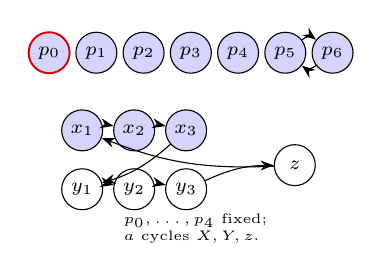
\begin{tikzpicture}[x=.60cm,y=.68cm,>=Stealth,
 state/.style={circle,draw,inner sep=1pt,minimum size=5.2mm,font=\scriptsize},
 active/.style={state,fill=blue!17},
 protected/.style={active,draw=red!85!black,line width=.7pt}]
\node[protected] (p0) at (0,0) {$p_0$};
\foreach \k in {1,...,6} {\node[active] (p\k) at (\k,0) {$p_{\k}$};}
\foreach \k in {1,...,3} {\node[active] (x\k) at ({1.1*(\k-1)+.7},-1.45) {$x_{\k}$};}
\foreach \k in {1,...,3} {\node[state] (y\k) at ({1.1*(\k-1)+.7},-2.55) {$y_{\k}$};}
\node[state] (z) at (5.2,-2.1) {$z$};
\draw[->,bend left=38] (p5) to (p6);
\draw[->,bend left=38] (p6) to (p5);
\foreach \u/\v in {x1/x2,x2/x3,y1/y2,y2/y3,x3/y1,y3/z,z/x1}
 {\draw[->] (\u) to[bend left=12] (\v);}
\node[font=\tiny,align=left] at (3.1,-3.28) {$p_0,\dots,p_4$ fixed;\\$a$ cycles $X,Y,z$.};
\end{tikzpicture}
\end{minipage}
\begin{minipage}{0.49\linewidth}
\centering{\small (b) Letter $b$}\\[-1pt]
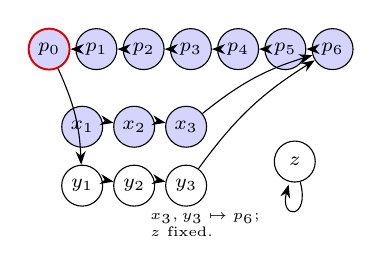
\begin{tikzpicture}[x=.60cm,y=.68cm,>=Stealth,
 state/.style={circle,draw,inner sep=1pt,minimum size=5.2mm,font=\scriptsize},
 active/.style={state,fill=blue!17},
 protected/.style={active,draw=red!85!black,line width=.7pt}]
\node[protected] (p0) at (0,0) {$p_0$};
\foreach \k in {1,...,6} {\node[active] (p\k) at (\k,0) {$p_{\k}$};}
\foreach \k in {1,...,3} {\node[active] (x\k) at ({1.1*(\k-1)+.7},-1.45) {$x_{\k}$};}
\foreach \k in {1,...,3} {\node[state] (y\k) at ({1.1*(\k-1)+.7},-2.55) {$y_{\k}$};}
\node[state] (z) at (5.2,-2.1) {$z$};
\foreach \j in {1,...,6} {\pgfmathtruncatemacro{\prev}{\j-1}\draw[->] (p\j) to (p\prev);}
\foreach \u/\v in {p0/y1,x1/x2,x2/x3,y1/y2,y2/y3,x3/p6,y3/p6}
 {\draw[->] (\u) to[bend left=11] (\v);}
\draw[->] (z) edge[loop below] (z);
\node[font=\tiny,align=left] at (3.3,-3.28) {$x_3,y_3\mapsto p_6$;\\$z$ fixed.};
\end{tikzpicture}
\end{minipage}
\caption{A complete 14-state binary witness. Only the $a$-loops at $p_0,\ldots,p_4$ are suppressed. The word $a^6ba^3b$ compresses at length 11; $a^6bab^5$ omits $p_0$ at length 13. The drawing gives the actual letter transformations, not a quotient automaton.}
\label{fig:witness}
\end{figure}

\section{The sharp binary lower-bound construction}
\begin{theorem}\label{thm:two-block}
Put $m=n-s\ge3$ and $q=n-r\ge2m+2$.
There is a binary strongly connected synchronizing automaton with reachable
$S$ attaining $\ac(S,A)=\min\{q,3m-1\}$.
Consequently $\Max_{\rm bin}=\Max=q$ whenever $2m+2\le q\le3m-1$.
For larger $q$ the construction gives only a lower bound.
\end{theorem}
\begin{proof}
Write $t=m-1\ge2$ and $p=n-2t-1\ge r+3$.
Take $P=\{p_0,\ldots,p_{p-1}\}$, $X=\{x_1,\ldots,x_t\}$,
$Y=\{y_1,\ldots,y_t\}$ and one further state $z$.
Letter $a$ interchanges the last two $P$-states, fixes the others, and
cycles $x_1,\ldots,x_t,y_1,\ldots,y_t,z$.
Letter $b$ sends $p_0$ to $y_1$, $p_i$ to $p_{i-1}$ for $i\ge1$,
increments indices in $X,Y$ below $t$, sends both $x_t,y_t$ to $p_{p-1}$,
and fixes $z$. Put $S=P\cup X$, $A=\{p_0,\ldots,p_{r-1}\}$ and $L=3t+2$.

\emph{No compression before $L$.}
For $\rho_i=\min\{i,p-2\}$ define a symmetric potential $\Phi$ on unordered
pairs, zero on singleton pairs, by the following table. Indices in $X,Y$
run from $1$ to $t$, and indices in $P$ from $0$ to $p-1$.
\begin{center}\small
\begin{tabular}{ll}
pair&potential\\ \hline
$P$--$P$, $P$--$X$, $X$--$X$ (distinct)&$L$\\
$\{x_i,y_j\}$, $j=i$&$t-i+1$\\
$\{x_i,y_j\}$, $j>i$&$2t-i+1$\\
$\{x_i,y_j\}$, $j<i$&$L-j$\\
$\{x_i,z\}$&$2t-i+1$\\
$\{y_i,y_j\}$, $i<j$&$L-j$\\
$\{y_i,z\}$&$2t+1$\\
$\{p_i,y_j\}$&$\min\{L,\max\{L-j,2t+3+\rho_i\}\}$\\
$\{p_i,z\}$&$\min\{L,2t+2+\rho_i\}$
\end{tabular}
\end{center}
Substitution in the two letter actions gives
\[
 \Phi(E)\le1+\Phi(Ea),\qquad \Phi(E)\le1+\Phi(Eb).
\]
Here are the boundary checks. The last-two-$P$ interchange preserves $\rho$;
a downward $P$-step decreases it by at most one.
For $P$--$Y$ pairs the $a$-boundary $y_t\to z$ decreases the second term
from $2t+3+\rho$ to $2t+2+\rho$.
The $b$-boundary $p_0\to y_1$ with $j<t$ has source $L-j$
and target $L-j-1$, since $j\le t-1$; with $j=t$ its target is at least $L-1$.
For $X$--$Y$, crossing $x_t$ under $a$ gives $Y$--$Y$ with potential $L-j-1$
when $j<i$; crossing under $b$ gives $P$--$Y$ of at least that potential.
The kernel pair $\{x_t,y_t\}$ has potential one.
Crossing $y_t$ in a $Y$--$Y$ pair under $a$ gives $Y$--$z$ of
potential $2t+1=L-t-1$.
For $X$--$z$, the $a$-boundary is $\{x_t,z\}\to\{y_1,x_1\}$,
with values $t+1,t$; for $Y$--$z$, every $a$-image has potential $2t$.
All remaining cases either retain potential, decrement an index by one,
or enter a type whose potential is at least the source minus one.
Clipping at $L$ cannot increase a positive difference.
Thus the inequalities hold for every index, not just tested sizes.
Every distinct pair in $S$ has potential $L$.
Telescoping along a merging word proves its length is at least $L$;
every compression merges an initial pair, giving the claimed lower bound.

\emph{No avoidance before $q$.}
Use singleton $P$-cells and $t$ color cells, giving $x_i,y_i$ color $i$
and $z$ color $1$. Let $T_a$ swap the last two $P$-cells and cycle the colors,
and let $T_b$ cycle $p_0,1,\ldots,t,p_{p-1},\ldots,p_1$.
For the incidence matrix $C$ both letters satisfy
\[
 D_\ell C=CT_\ell+f_z(e_1-e_2).
\]
Here $D_\ell$ is the original-letter transition matrix, $f_z$ the $z$-column, and $e_i$ the color row; the displayed discrepancy is a rank-one outer product.
Since $S$ has one state in every cell, induction along each original word $w$ gives
$\chi_S D_w C=\mathbf1+\sum_j\mu_j(e_1-e_2)T_{w_j}$,
where $\mu_j\ge0$ counts trajectories at $z$ immediately before the corresponding suffix $w_j$.
A trajectory from $X$ needs at least $t+1$ steps to reach $z$;
any entrance from $P$ starts at $y_1$ after at least one step and then needs
at least $t$ more. Thus the first nonzero correction has position at least $t+2$.
In the prescribed cell graph, color $2$ needs $t-1$ letters to enter $P$
at $p_{p-1}$ and at least $p-r$ more to reach $A$.
The only interchange is between adjacent last $P$-points and cannot shorten
this descending path. A negative correction therefore reaches $A$ only at
length at least $(t+2)+(t-1+p-r)=p+2t+1-r=q$.
Before then every protected coordinate has multiplicity at least one.

\emph{Attainment.}
After $a^{2t}b$, the missing $P$-point is $p_{p-1}$; after a further $a$
it is $p_{p-2}$. This is the unique $b^{p-r-1}$-preimage of $p_{r-1}$.
Hence $a^{2t}bab^{p-r-1}$ omits that protected point at length $q$.
The $X\cup Y\cup\{z\}$ portion after $a^{2t}b$ is
$\{x_2,\ldots,x_t,y_1,z\}$. After $a^t$ it contains $x_t$ and $y_t$,
so $a^{2t}ba^tb$ compresses at length $L$.
The existence of $x_t$ in the preceding set uses $t\ge2$.
Combining both upper witnesses with the lower bounds gives $\ac(S,A)=\min\{q,L\}$.

\emph{Structural requirements.}
Put $B=P\cup Y$, $h=p+t$ and $E=B\cup\{z\}$.
Letter $b$ cycles $B$ in the order $p_0,y_1,\ldots,y_t,p_{p-1},\ldots,p_1$,
and $Qb^t=E$. The $a$-cycle connects all other states to $B$, proving
strong connectivity.
On $E$, $d=a^{2t}b^h$ fixes $P$, cycles $y_1\to y_t\to\cdots\to y_1$,
and sends $z$ to $y_t$. Thus $e=d^t$ fixes $B$ and sends $z$ to $y_1$.
Since $Ba^{t+1}=S$, the original-letter word $b^tea^{t+1}$ reaches $S$.
The word $a^{2t+1}$ fixes $X\cup Y\cup\{z\}$ and transposes the last two
$P$-points, adjacent on the $b$-cycle. These words generate every permutation
of $B$, with inverses realized by positive powers.
Moreover $Ba=(B\setminus\{y_1\})\cup\{z\}$,
$Bab=(B\setminus\{y_2\})\cup\{z\}$, and $Babe=B\setminus\{y_2\}$.
Permutations route any pair in a current image into the kernel of $abe$;
repeated compression synchronizes $B$. Prepending $b^te$ synchronizes $Q$.
Finally $L=3m-1<\binom{m+2}{2}$ for $m\ge3$, so meeting $q\le L$
determines both maxima as stated.
\end{proof}



\section{The short-pair graph and the route to upper bounds}\label{sec:method}

Let $P_h$ join two distinct states if an original-letter word of length at most $h$ merges them; write $\tau(P_h)$ for its minimum vertex cover. A set $T$ of size $n-m$ survives pure compression through depth $h$ precisely when it is independent in $P_h$. Consequently
\begin{equation}\label{eq:cover}
\exists T,\ |T|=n-m,\ c(T)>h\quad\Longleftrightarrow\quad \tau(P_h)\le m.
\end{equation}
The graph keeps the \emph{global} automaton state identity. We use the Frankl--Pin compression framework and its short-pair refinement~\cite{kisielewicz2016}. It is not permitted to replace different unnamed states separately for each input letter. This is the starting point of both computer-assisted upper bounds.

The reductions first bound the nonisolated support of an early short-pair layer, then enumerate its graph isomorphism classes and later maximal independent-set families. Every original input letter yields a row of a finite \emph{necessary relaxation}; joint row- and pair-merging distances, common-state quotient connectivity and same-letter square constraints yield further necessary restrictions. These necessary constraints may admit spurious finite models. They are used in only one direction:
\[
\text{a genuine counterexample}\ \Longrightarrow\
\text{a compatible necessary-domain model}.
\]
Thus a complete UNSAT enumeration gives an upper bound, whereas SAT by itself does \emph{not} yield an automaton.

\subsection{Defect four: excluding twelve steps}\label{sec:m4}
Suppose $n\ge11$, $|S|=n-4$, and $c(S)\ge12$. The complete short-pair reduction splits at depth seven:
\begin{enumerate}
\item $\tau(P_7)\ge4$: all remaining candidates lie in 91 graph cores; the finite letter/distance search excludes each.
\item $\tau(P_7)=3$: the paper reduction yields $\tau(P_9)=4$ and 117 graph classes with 10,142 named necessary domains. The complete compatible-letter and joint-distance checks exclude them all.
\end{enumerate}
The enumeration is independent of a bound on $|\Sigma|$; it enumerates the full admissible original-letter pools and requires common realizability as a \emph{necessary} condition. This establishes $c(S)\le11$. At $n\le10$, the universal avoid-or-compress bound $q\le9$ suffices. Binary witnesses from Theorem~\ref{thm:two-block} ($q\ge10$) and Proposition~\ref{prop:smallq} ($q=5,\ldots,9$) complete the equality. The complete case reductions appear in the fixed original record~\cite{repo}; current program locations and verification obligations are collected in the companion \href{https://github.com/dongxuelian2/cerny-direct-attack/blob/main/research/problem4/CERTIFICATES.md}{certificate map}.

\subsection{Defect five: excluding fifteen steps}\label{sec:m5}
Suppose $n\ge16$, $|S|=n-5$, and $c(S)\ge15$. The relevant split is $\tau(P_9)=5$ or $4$.
\begin{center}\small
\begin{tabular}{@{}p{.30\linewidth}r p{.35\linewidth}@{}}
\toprule
Necessary branch & Domains/cores & End state of exclusion\\\midrule
Cover five & 2,294 cores & all rejected by joint necessary checks\\
Cover four, 11-point early support & 90 cores, 3,595 domains & disjoint completed checks and auxiliary-source lemma\\
Cover four, support 5--10 & 4,568 cores, 3,245,386 domains & 38,398 static rejections; 3,206,988 complete dynamic checks\\
\bottomrule
\end{tabular}
\end{center}
The final large run did \emph{not} return zero survivors. It reported 3,206,987 UNSAT domains and precisely one satisfying \emph{relaxation} domain: core 447, domain 0, whose ninth-layer graph on eight named states is $K_{4,4}$. Its four relevant later independent sets are
\[
\{0,1,2\},\quad\{0,1,3\},\quad
\{4,5,6\},\quad\{4,5,7\}.
\]
The following paper lemma rules out this remaining possibility.

\begin{lemma}[Multipartite overlap exclusion]\label{lem:multipartite}
Let $h\ge1$ and $t\ge2$. Suppose a noncomplete $P_h$ in a synchronizing automaton is a complete multipartite graph on $V=V_1\sqcup\cdots\sqcup V_t$ and has isolated remaining states $J$. Assume each $V_i$ admits a family $\mathcal R_i$ of nonempty subsets whose union is $V_i$, whose intersection graph is connected, and for which every $R\cup J$ with $R\in\mathcal R_i$ is independent in $P_{h+1}$. Then this configuration is impossible.
\end{lemma}
\begin{proof}
A $P_h$ nonedge cannot be merged in one letter. Fix a letter $f$. It is therefore injective on each part and on $J$, and $Jf$ is disjoint from $Vf$. Since every $(R\cup J)f$ is $P_h$-independent, if $Jf\subseteq J$, then $Jf=J$ and $Rf$ is contained in some single part. Intersecting $R,R'$ have intersecting images, so the connected intersection graph forces all of $V_if$ into one part. Every original nonedge remains a nonedge.

Otherwise $Jf$ meets some part $V_j$. Independence of $(R\cup J)f$ forces $Rf\subseteq V_j\cup J$ for every $R$, hence $Vf\subseteq V_j\cup J$ and $Jf\subseteq V_j\cup J$. Again every original nonedge remains a nonedge. This holds for every letter. But a synchronizing automaton with noncomplete $P_h$ must have some letter sending a nonedge to an edge of $P_h$: follow the shortest merging word for a pair at distance greater than $h$ until the distance first drops from $h+1$ to $h$. Contradiction.
\end{proof}
The two pairs of intersecting triples above separately cover the two parts of $K_{4,4}$, and their rows (with common isolates adjoined) are independent in $P_{11}$, hence in $P_{10}$. Lemma~\ref{lem:multipartite} with $h=9$ excludes the only relaxation survivor. Thus the combined complete finite exclusions establish $c(S)\le14$. For $n\le15$, the original bound $q\le14$ suffices. Matching binary witnesses are given by Theorem~\ref{thm:two-block} for $q\ge12$ and Proposition~\ref{prop:smallq}: the first and second cardinality faces cover $q=6,7$, and the cofinal construction covers $q=8,\ldots,11$.

\section{Auxiliary results and remaining question}\label{sec:conj}
The same research establishes a restricted-class result for automata with an original full-state cycle letter:
\[
\Max_{\mathrm{cyc,bin}}(n,s,r)=\Max_{\mathrm{cyc}}(n,s,r)
=\min\{s-r+1,\,2(n-s)+1\}.
\]
This has a paper binary construction for all legal parameters; it is not an unrestricted upper bound. A quadratic lifting argument additionally selects at most $\rho\le\min(|\mathcal D|,d_{\mathcal D}(d_{\mathcal D}+1)/2)$ original letters preserving all exact shortest exits of a \emph{complete} safe-set family $\mathcal D$. Here $d_{\mathcal D}=\dim_{\mathbb Q}\operatorname{span}\{\chi_T:T\in\mathcal D\}$ is its characteristic-row rank and $\rho=\dim_{\mathbb Q}\operatorname{span}\{\chi_T^{\mathsf T}\chi_T:T\in\mathcal D\}$ is its quadratic-lift rank. Neither auxiliary theorem is a hidden dependency for the exact defect-five exclusion.

The binary construction gives the lower bound $3m-1$ for every $m\ge4$ when $q$ is large. At $m=4,5$ we have matching upper bounds. Restricted families at $m=6,7$ attain the values 17 and 20; local and random counterexample probes have found no larger instances, but these finite results are \emph{not} general upper bounds.
\begin{conjecture}[Linear defect bound; unproved]\label{conj:linear}
For every $m\ge4$ and all admissible $n,r$,
\[
\boxed{\Max_{\rm bin}(n,n-m,r)=\Max(n,n-m,r)=\min(n-r,3m-1).}
\]
\end{conjecture}
The restriction $m\ge4$ is essential: at $m=3$ the known optimum is $\min(q,9)$, whereas $3m-1=8$. A \emph{stronger and distinct} possible bound would assert $c(S)\le3m-1$ for every $(n-m)$-subset when $n\ge3m+1$; we do not assert equivalence with Conjecture~\ref{conj:linear}. The unknown exact-extremum range starts at $m\ge6$, $q\ge3m$.

\section{Proof provenance and audit status}\label{sec:audit}
The paper establishes a linear dependency chain and describes the finite exclusion logic, but the detailed family classification and software specifications are in the permanent Git research record~\cite{repo}. The formerly mixed 2.85 MB working notebook is preserved unchanged in the archival folder, while a dedicated \href{https://github.com/dongxuelian2/cerny-direct-attack/tree/main/research/problem4}{Open Problem 4 reader index (PR \#15)} records proof dependencies, source paths and an audit checklist. The largest defect-five run, a 3,206,988-domain computation of about 22,924 seconds, was reported complete from an owner's terminal summary but its comprehensive raw log or a portable per-domain proof certificate is not committed. Its two generator orders share tests, so they do not constitute independent formal proof systems. The present research manuscript should therefore be read as a \emph{computer-assisted proof with documented verification gaps}, pending an external audit. No extension of the unrestricted result to all $m$ or of the \v{C}ern\'y conjecture is claimed.

\paragraph{Contributions and assistance.} The work reflects research by Qichao Wang and Daoyu Dong, with computational and AI-assisted proof exploration and drafting. Mathematical responsibility and claims of priority remain subject to author review.

\begin{thebibliography}{9}
\bibitem{szykula2018} M. Szyku{\l}a,
\emph{Improving the Upper Bound on the Length of the Shortest Reset Word},
STACS 2018, LIPIcs 96, 56:1--56:13.
\href{https://doi.org/10.4230/LIPIcs.STACS.2018.56}{DOI}.
\bibitem{szykula2026} M. Szyku{\l}a,
\emph{Synchronizing Automata: Open Problems},
EPTCS 451 (2026), 33--47.
\href{https://doi.org/10.4204/EPTCS.451.3}{DOI}.
\bibitem{kisielewicz2016} A. Kisielewicz, J. Kowalski, and M. Szyku{\l}a,
\emph{Experiments with Synchronizing Automata},
CIAA 2016, LNCS 9705.
\bibitem{repo} Q. Wang and D. Dong,
\emph{Original research record for dense-subset avoid-or-compress},
\href{https://github.com/dongxuelian2/cerny-direct-attack/tree/cc94b58aa9b557f0ee516b3a3774de3ad8e41de1}{fixed record at merged PR \#14}; the later \href{https://github.com/dongxuelian2/cerny-direct-attack/pull/15}{PR \#15} contains the editorial audit,
20 October 2026.
\end{thebibliography}
\end{document}
